\chapter{Background}

\label{chap:background}
In this chapter, we introduce the technology of Wireless Sensor Networks, the Chaos protocol, the \atwo{} system, and gossiping protocols. Furthermore, we explain what clustering is and provide insight into different objectives when clustering to a network. Finally, we present a categorisation of properties for clustering algorithms.


\section{Wireless Sensor Networks}
A \emph{Wireless Sensor Network} (WSN) consists of many small low powered computer nodes equipped with sensors, cooperatively working towards a goal. Typical applications include target tracking for the military, monitoring the weather, and tracking natural disasters \cite{Yick2008-wsn-survey}. There are several characteristics of a WSN that introduces challenges. However, they are also at the core of what makes WSNs useful. Examples of these characteristics are the low power nature and ad hoc deployment of the nodes. A typical node consists of four hardware units: sensors, processor, radio, and power \cite{Akyildiz2002-wsn-survey}, there can also be additional units for generating power or sensing its location. 

One of the primary objectives of a node is to preserve as much battery power as possible. Therefore, the hardware often has limited capabilities, restricting both the radio communication range and the processing power \cite{NikolaosA.Pantaziz2007-wsn-power-survey}. An example of a node that we use in this thesis is TMote Sky \cite{tmotesky-datasheet}, which has a CPU speed of 8MHz, 10KB RAM, and 48KB of flash storage. There are several ways to measure the lifetime of a WSN, and a typical measurement is the time until the first node has used up all its energy reserves and powers down. However, other measurements include the time until at least one node loses connection with the network, time until the network loses connection with a base station, or when a percentage of nodes have powered down.


Since the nodes are deployed in an ad hoc manner and use restricting hardware, an essential aspect of any protocol running on a WSN is fault tolerance. The protocol has to be able to handle a variety of failures such as packet loss due to interference or transmission error, node failures due to battery depletion, or other transient faults \cite{Mahmood2015-reliability-survey}. Moreover, in multi-hop networks that require forwarders, packets pass through several nodes, increasing the probability for these failures to occur before reaching the intended destination. There are two primary categories for achieving fault tolerance in WSN protocols: retransmission and redundancy \cite{Mahmood2015-reliability-survey}. In a protocol based on retransmission, each node waits for an acknowledgement of each packet it sends; if it receives none, the node will retransmit the packet. A protocol based on redundancy, on the other hand, includes extra bits in the packet which are used to detect, and sometimes even correct, faulty bits in any packets received.



\section{Chaos}
The Chaos protocol is the first WSN protocol that supports native all-to-all communication without sequential phases for collection, processing, and dissemination of information \cite{chaos-introduction-paper}. Traditionally, every node in the network schedules these phases at the same time, even if some nodes do not require it. In Chaos, on the other hand, every node independently decides what action to perform (transmit or receive data). However, all nodes perform one of these actions at the same time to enable them to communicate with each other without a central coordinator; this is called synchronous transmissions.


The smallest time component in the Chaos protocol is a \textit{slot}, in which every node performs one of two actions: transmit or receive. At the end of a slot, every node decides what their action will be in the next slot.
A node will transmit in the subsequent slot if it receives a packet with less or more information than itself. In the first case, it tries to spread its information to the node which sent a packet with less information. In the other case, a node merges the new information with its local data and then transmit in the next slot. A node will listen in the next slot if one of three scenarios happened in the previous slot: if it was transmitting, if it did not receive a packet, or if it received a packet but the packet did not contain any new information. 

Next, Chaos combines multiple consecutive slots to create a \textit{round}. During one round, Chaos executes one application. For example, the Max application in which all nodes spread their ID across the network and the merge operator executed on packet reception returns the maximum between the received number and a nodes local state. The number of slots in a round depends on the network size, a network with more nodes requires more slots.

\begin{figure}[bt]
    \centering
    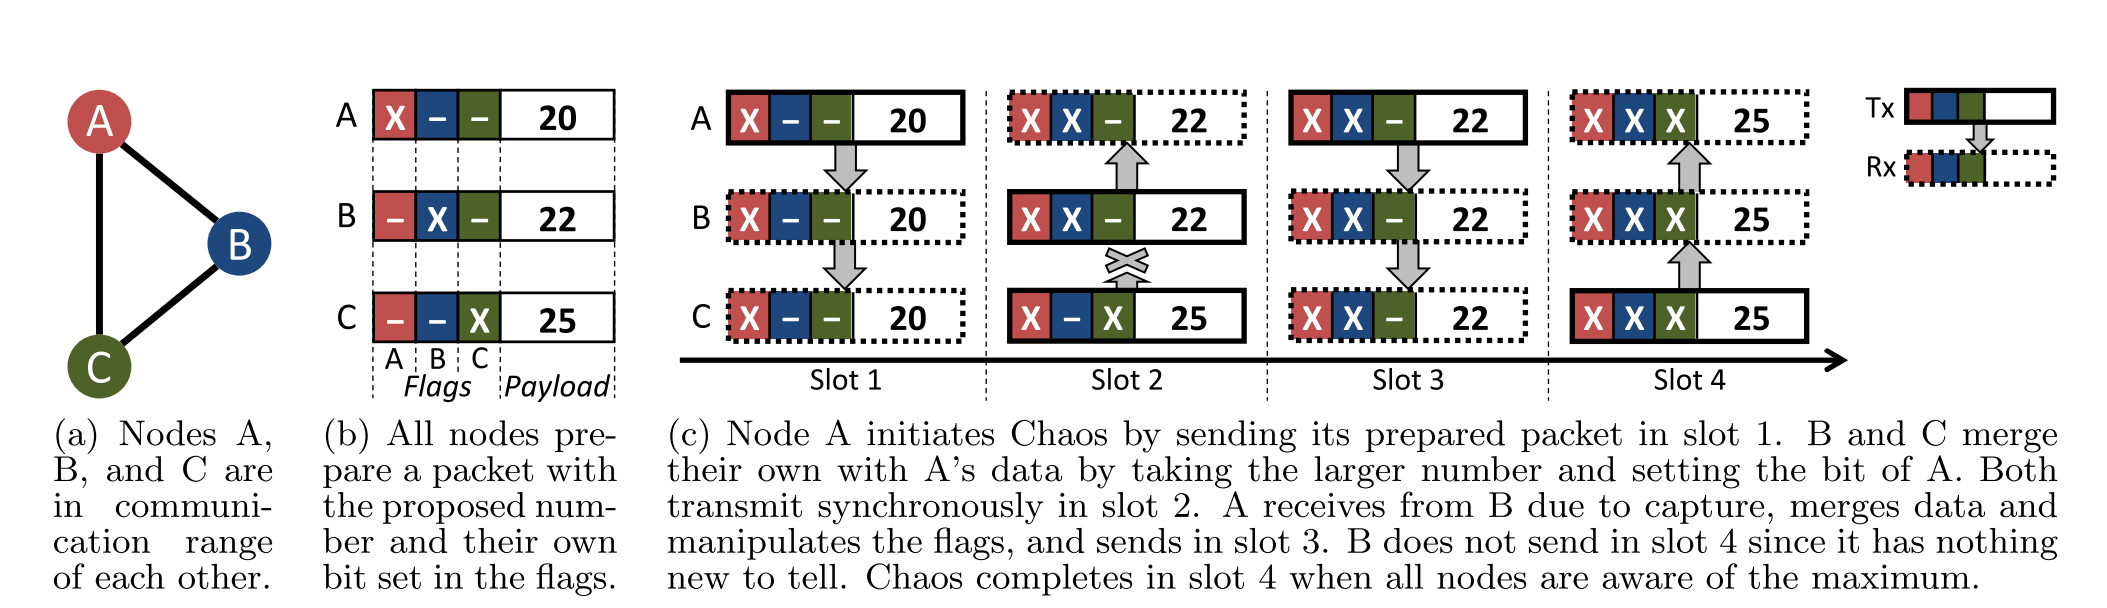
\includegraphics[width=\textwidth]{figure/ChaosOverview.png}
    \caption{An example of a Chaos round were three nodes reach consensus on the maximum of three proposed values \cite{chaos-introduction-paper}.}
    \label{fig:chaos-overview}
\end{figure}

\subsection{Synchronous Transmission}
Synchronous transmissions mean that all nodes execute rounds and slots at the same time. In \cref{fig:chaos-overview} time progresses towards the right, and we see that all slots are aligned. This transmission scheme enables Chaos to benefit from two physical phenomena:

\paragraph*{The capture effect} occurs when packets are colliding (received at the same time by one node). If one signal is at least 3dBm stronger and the timing between the packets are within a certain threshold, a node will correctly decode the stronger signal, and ignore the weaker one \cite{Lee2007-capture-effect}. Due to this effect, if a node receives two transmissions at the same time, one of them will, with high probability, be decoded correctly.

\paragraph*{Constructive interference} occurs when multiple nodes are transmitting the same packet at the same time. If that happens, the resulting signal strength is increased, which increases the probability that the packet will be received correctly by listening nodes.

\subsection{The Initiator}
In Chaos, a preconfigured node called \emph{the initiator} needs to be present, node \textit{A} in \cref{fig:chaos-overview}. The initiator is the node which initiates communication in a round. It also determines parameters such as what application to run and timing parameters for slots and rounds. All other nodes exclusively listen for packets until one is received which has propagated from the initiator. Both when the network boots up, and at the beginning of every round.

\subsection{Association}
When the network is booting, the nodes perform a process called association. During this time all nodes, except for the initiator, constantly listens while randomly choosing the radio channel, until they receive a packet with which they can synchronise. From this packet, a node learns timing parameters, the next application, slot, and round number. A node will also enter association when it has not received a valid packet for a configurable number of rounds, depending on the application that is running in the network.

\subsection{Flags Field}
\label{subsec-flags-field}
The \textit{flags field} is used by a node to keep track of which nodes have contributed during a round. It is a list of boolean values and can be seen in \cref{fig:chaos-overview}, marked as \textit{flags}. Each node in the network corresponds to an index in the list. At the start of a round, the initiator sets the value at its index to true. As packets propagate through the network, other nodes also set the value of their indices to true. Once a node has merged a received packet which sets all values in the flags field to true it knows that all nodes in the network have participated and the information it has is a complete view from the network.

The Chaos protocol has a limitation to its scalability due to the flags field. Since every node requires a 1-bit space in the flags field, if there is an upper limit on the packet size imposed by either the link-layer protocol or the nodes, the number of nodes in the network is limited by the maximum size of the packet. 

\subsection{Completion Flooding}
\emph{Completion flooding} is executed at the end of a round if a node notices that all flags in the packet are set to true. Once in this phase, the node broadcasts its completed packet every other slot for a configurable number of slots. Aggressively transmitting the packet causes neighbouring nodes to reach completion which causes them to enter the completion phase. Since all nodes in this phase broadcast the same packet, the signal benefits from constructive interference which makes the signal of the complete packet stronger causing the capture effect to apply more often.

\subsection{Timeout Mechanism}
To prevent premature termination a \textit{timeout mechanism} triggers if a node has not received a packet for some number of slots. Premature termination is when some nodes do not have all the information, but the communication has stopped. The number of slots is selected randomly by each node from an interval. When a node reaches that timeout, the node transmits a packet. If nearby nodes see that a node near them has less information than they do, they will transmit in the next slot, and thus communication is restarted.

\section{Agreement in the Air}
\label{sec:chaos-a2-background}
As the original implementation of Chaos has much potential, further research conducted by Al Nahas et al.~\cite{a2-introduction-paper} resulted in the \atwo{} Synchrotron. \atwo{} is a layer that provides services to the application layer, as seen in \cref{fig:original-a2-architecture}. The Synchrotron kernel is a further development of Chaos. In this section we, First, describe the scheduler in Synchrotron. Second, we cover the dynamic group membership provided by \atwo{}'s Join and Leave services. Last, we explain how Synchrotron achieves frequency agility with parallel channels and channel hopping. The remaining architecture description shown in \cref{fig:original-a2-architecture} is explained in \cite{a2-introduction-paper}.

\begin{figure}[bt]
    \centering
    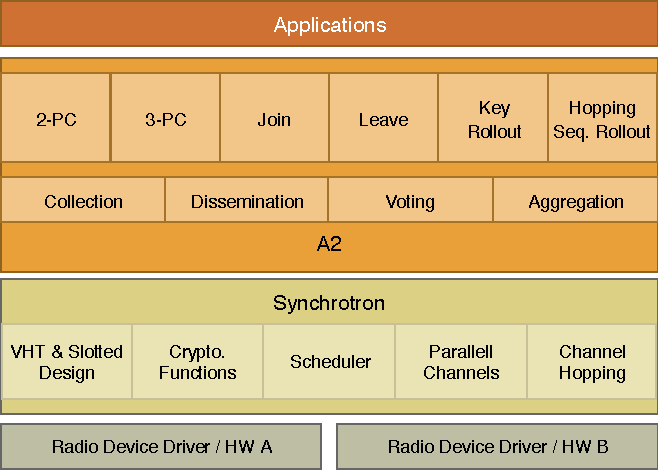
\includegraphics[scale=0.7]{figure/architecture_original_a2.pdf}
    \caption{The original \atwo{} architecture \cite{a2-introduction-paper}.}
    \label{fig:original-a2-architecture}
\end{figure}

\subsection{The Scheduler}
The scheduler in \atwo{} allows the initiator to schedule multiple applications dynamically. During each round, the initiator sets a \textit{next app} field in the packet to instruct the rest of the network which app should run in the next round. With the scheduler, a network can run multiple applications or services at different intervals, without any interference between applications. The scheduler also facilitates the scheduling of the dynamic group membership, scheduling the Join and Leave services as needed when nodes either request to join or disappear from the network.

\subsection{Dynamic Group Membership}
\label{background-a2-join-service}
Dynamic Group Membership is implemented using the Join service, which allows the network to assign indices for nodes in the flags field dynamically. A node wanting to join the network sets the join flag in the packet header. Once the initiator receives a packet with a join flag, in say round $r$, it will in round $r + 1$ tell all nodes to schedule the Join service for round $r + 2$. The join round runs in two phases, collect and disseminate. We show an example of the Join service with three nodes in \cref{fig:join-service-overview}.

\begin{figure}[bt]
    \centering
    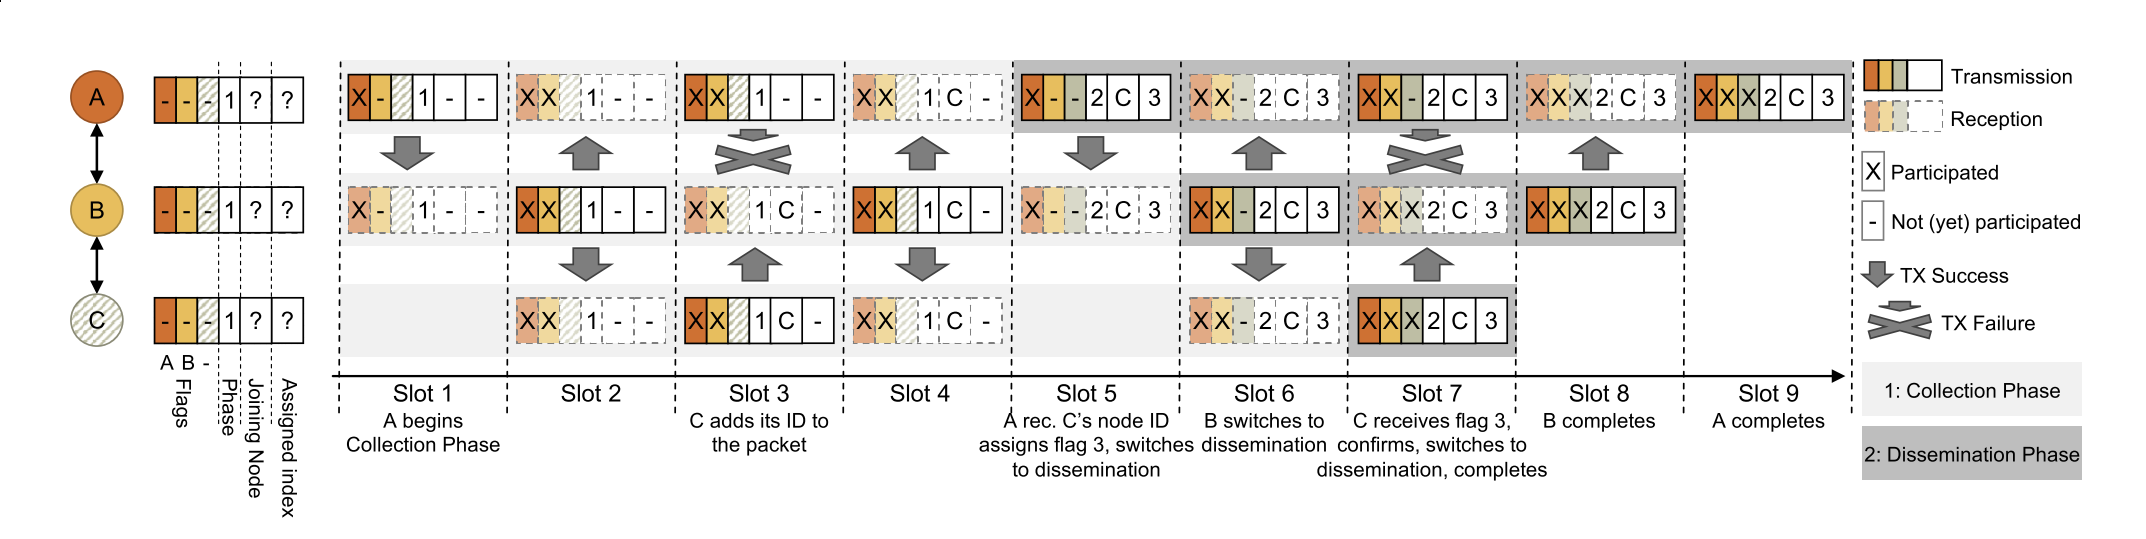
\includegraphics[width=\textwidth]{figure/JoinServiceOverview.png}
    \caption{The Join service exemplified using three nodes \cite{a2-introduction-paper}.}
    \label{fig:join-service-overview}
\end{figure}

\paragraph*{The Collect Phase} is the first phase, where the network constructs a list in which nodes that want to join the network adds their node ID. The initiator will switch to the second phase (Slot 5 in \cref{fig:join-service-overview}) when it notices full participation of the network and does not record any changes to the join list for a couple of slots, or if the list is full.

\paragraph*{The Disseminate Phase} is the second phase, where the initiator assigns each new node an index in the flags field. The initiator then disseminates the join list with updated information about the joining nodes flag indices. Each joining node can now set the flag in their index as an acknowledgement (C sets its flag in Slot 7). In case a node misses the dissemination, it will request another join round and be assigned the same flag index again.

The Leave service removes nodes from the flags field if they do not participate for a set number of rounds. When it triggers, a join round is scheduled to disseminate the information about what nodes are present. The Leave service ensures that disappearing nodes does not hinder the completion phase.

\subsection{Frequency Agility}
\label{subsec-frequency-agility}
In the presence of interference, the performance of \atwo{} degrades. Al Nahas et al.~solves this by introducing frequency hopping and parallel channels.

\paragraph*{Frequency hopping} consists of each node switching which radio channel they use to transmit and receive data in unison in every slot. By switching channels, using the default hopping sequence from the IEEE 802.15.4e standard \cite{IEEE-802-15-4}, the network avoids interference from other network traffic, which might occupy a single channel, allowing \atwo{} to exist side-by-side with other wireless systems. 

\paragraph*{Parallel Channels} alleviates the issues caused by having a dense network with many nodes transmitting simultaneously in the same area. Many simultaneous transmissions on the same frequency cause interference, which damages the probability of packet capture. Synchrotron allows for a configurable number of channels from which nodes pick randomly in each slot to use for reception or transmission. The number of parallel channels require configuration and could damage the performance of a network if it is set too high or low.


\section{Gossiping}
\begin{newtext}
Gossiping, presented by Demers et al.~\cite{Demers1987-gossiping-first-paper} in 1987, is an effective and straightforward method for disseminating updates throughout a large distributed system. Gossip algorithms are also called epidemic algorithms since they work similarly to how diseases spread, thus, gossiping borrows some terminology from epidemiology. For example, a node with new information is infective, and a node unaware of that update is susceptible to that node. Gossip algorithms spread updates using elementary actions called push and pull. One common problem is that nodes cannot know when the network has reached consensus; however, networks that use gossip protocols have eventual consistency.

During one gossiping round, a node either pushes or pulls updates from a uniformly random selected node. Both actions are required to infect all nodes effectively; the argument for this is intuitive: Consider a network with $n$ number of nodes. A new update originating at node $u$ is hard to find for all other nodes since the probability to select $u$ is $\frac{1}{(n-1)}$. However, if $u$ decides to use the push action, it is sure to infect another node. Moreover, as the number of infected nodes grows to more than $\frac{n}{2}$, the push action has less than 50\% probability of infecting a susceptible node. However, the susceptible nodes have greater than 50\% probability of selecting an infected node when they use the pull action.

Using a push and pull scheme to spread updates throughout a distributed system is effective. However, if the nodes in the system communicate using direct communication in every round, a gossiping algorithm cannot achieve both time- and communication-optimality \cite{Karp2000-randomized-rumour-spreading}, that is, completing in only $\mathcal{O}(log\,n)$ rounds using only $\mathcal{O}(n)$ messages. Karp et al.~\cite{Karp2000-randomized-rumour-spreading} investigate this problem, and they show that every algorithm that spreads a rumour in $\mathcal{O}(ln\,n)$ rounds needs $\mathcal{\omega}(n)$ transmissions, where $n$ is the number of nodes in the system.

In further developments of gossiping protocols, it is possible for nodes to only have a partial view of the network, called a group, as described by Eugster et al.~\cite{Eugster2004-epidemic-information-dissemination-in-distributed-systems}. Every message sent is \emph{piggybacked} with information about what nodes the transmitter knows about, allowing a receiver to update its membership group dynamically, replacing some nodes in its group with some of the newly received ones to maintain an average group size. When a new node wants to join the network, it contacts either an arbitrary or dedicated node, which is called the bootstrapping node. The bootstrapping node first decides if it should save the new node to its group and then forwards the information about the new node to its group members. Each member then repeats the same process recursively up to a configured depth, which depends on the size of the group. The new node initialises its group with the bootstrapping node and then add nodes to its group dynamically using the information that is piggybacked in every packet.

Only maintaining a partial view of the network improves scalability as it, in larger networks, becomes infeasible for a node to maintain information about all nodes. In exchange for scalability, the algorithm loses reliability. The reason for this is that the larger the view of the network a node has, the less the risk is for partitioning to occur  \cite{Eugster2004-epidemic-information-dissemination-in-distributed-systems}.


\end{newtext}

\section{Clustering}
\label{sec:background:clustering}
Clustering is the task of partitioning a network and electing nodes, called Cluster Heads (CH), which are responsible for a network-wide communication overlay \cite{Younis2006-clustering-survey}. All other nodes only communicate within their cluster. Each CH retains information from its cluster and forwards that to other CHs or a base station. A base station is not a sensor node; it is not battery powered and usually only collects data from other nodes. In some networks, there is no base station; the aim is instead to inform all nodes in the network of the calculated values. In either case, it is the job of the CH to make sure that the relevant parties get the final value.

A phenomenon that can occur when nodes or CHs are using a many-to-one communication pattern, such as when aggregating data to a base station, is the hot spot problem \cite{Perillo2005-hot-spot-survey}. Nodes that are closer to the base station will need to handle more network traffic, and this can lead to them depleting their energy earlier than other nodes in the network. In the worst case, this can cause the network to become cut off from the base station entirely, completely disabling the network.

Clustering can be beneficial in several aspects; we list some objectives of clustering in \cref{sec:clustering-objectives}. One of the most critical components of a WSN is its energy consumption and using the radio to transmit and receive data is generally the most expensive operation of a node \cite{Anastasi2009-wsn-energy-consumption}. Clustering has been shown to decrease the amount of communication, making clustering an excellent candidate to preserve energy in a WSN.


\subsection{HEED}
\label{subsection:background-heed}
In this thesis, we base our work on the HEED algorithm \cite{Younis2004-HEED}, a probabilistic algorithm with the primary objective of saving energy. To this end, HEED uses residual node energy as its main parameter to elect CHs and intra-cluster communication cost as its second parameter. An example of intra-cluster communication cost is the number of nodes that have already joined a cluster. In HEED, the clustering algorithm executes at regular intervals ranging from seconds to hours depending on the application the network is running and how significant the increase in energy consumption is for CHs.

At the start of the clustering algorithm, each node sets an initial probability to, for example, $C_{prob} = 5\%$. Then, the node applies its proportion of residual energy as weight according to

\begin{equation*}
CH_{prob} = C_{prob} * \frac{E_{residual}}{E_{max}}
\end{equation*}

to calculate its probability of becoming CH. Where $E_{residual}$ and $E_{max}$ is the residual energy and the maximum possible energy respectively. The value of $CH_{prob}$ is limited by a carefully selected lower bound, inversely proportional to the value of $E_{max}$ to ensure that the algorithm terminates in $\mathcal{O}(1)$ time. At the end of every iteration of the algorithm, this probability is doubled, until the algorithm terminates or $CH_{prob}$ reaches 1. 

Furthermore, there are two stages for any node announcing itself as CH; a node first becomes a \textit{tentative} CH until it either resigns or becomes a \textit{final} CH. A node announces itself as a tentative CH with probability $CH_{prob}$ if it has not heard from any other CH and becomes a final CH if $CH_{prob} = 1$. A CH resigns from being tentative if it finds another CH to join with lower cost than itself. Last, if a node reaches the end of the algorithm without hearing a final CH, it will announce itself as a final CH to ensure that CHs cover the whole network.



\section{Clustering Objectives}
\label{sec:clustering-objectives}
There are two categories of clustering objectives, primary and secondary, and when designing a clustering algorithm achieving one or more of the primary objectives is often the goal. In contrast, the secondary objectives are usually not targeted explicitly in the algorithm design, but instead often indirectly achieved when clustering the network \cite{Afsar2014-clustering-survey}. We list some common primary and secondary objectives in \cref{table:clustering-objective}.

\begin{table}[b]
\centering
\caption{An overview of primary and secondary clustering objectives \cite{Afsar2014-clustering-survey}.}
\label{table:clustering-objective}
\begin{tabular}{cc}
\multicolumn{2}{c}{{\textbf{Clustering Objectives}}}                   \\ \hline
\multicolumn{1}{c|}{\textbf{Primary}}            & \textbf{Secondary}      \\ \hline
\multicolumn{1}{c|}{Scalability}                 & Increased connectivity  \\
\multicolumn{1}{c|}{Fault-tolerance}             & Reduced routing delay   \\
\multicolumn{1}{c|}{Data aggregation/fusion}     & Collision avoidance     \\
\multicolumn{1}{c|}{Load balancing}              & Using sleep schemes \\
\multicolumn{1}{c|}{Stabilised network topology} &                         \\
\multicolumn{1}{c|}{Maximal network lifetime}    &                        
\end{tabular}
\end{table}

\subsection{Primary Clustering Objectives}
All the primary objectives are usually desired when implementing a clustering algorithm. However, it can be difficult to achieve all of them at the same time. There are often trade-offs between the objectives, and instead, it is common to only target a few of them.

\paragraph*{Scalability} is a consequence of clustering since the network is partitioned, making the network artificially less dense. Factors that need to be considered when designing for scalability include network density and routing delays.

\paragraph*{Fault tolerance} is often a requirement for mission-critical applications. A clustering algorithm can be fault tolerant by periodically reclustering the network. If a node dies and some part of the network loses connectivity, a reclustering can reconnect the network again.

\paragraph*{Data aggregation/fusion} is the act of filtering out redundant data at some point before it reaches its destination. If the application a WSN is running is only interested in the average, or otherwise redundant data is sent, the CH can filter out that data and decrease the number of packets transmitted.

\paragraph*{Load balancing} is achieved by periodically changing the nodes that are CHs. Assuming that being a CH requires more battery, load balancing will increase the total lifetime of the network since the CH role is distributed among all nodes.

\paragraph*{Stabilised network topology} concerns the mobility of nodes. If a node moves and switches cluster, the CH can register this change and keep the network topology up to date.

\paragraph*{Maximal network lifetime} is a common objective often, in part or entirely, caused by the other objectives. For example, proper load balancing means avoiding early node deaths, and data aggregation means the network can filter unnecessary traffic. Both of these properties work towards an energy efficient cluster which implies an extended network lifetime. 

\subsection{Secondary Clustering Objectives}
The secondary objectives are not usually a target when implementing clustering algorithms but rather achieved indirectly by targeting the primary objectives.

\paragraph*{Increased connectivity} is achieved since in a clustered network only the CHs need to be connected to each other. All other nodes only have to be connected to their cluster, which relaxes the requirement for a network to be considered fully connected.

\paragraph*{Reduced routing delay} is desired for some applications, packets need to arrive within a specified time limit; this can be a challenge in a widespread WSN. With clustering, the communication within a cluster can arrive faster since the clusters are smaller and closer together than the network as a whole.

\paragraph*{Collision avoidance} is achieved since transmission collisions may cause packet loss, which is energy wasted on doing nothing. To minimise packet loss, clusters can split their communication between different radio channels or different time slots.

\paragraph*{Using sleep schemes} can be beneficial since in some applications there is no need for the whole network to be active all the time. For example, some nodes might only provide routing paths. In this case, all paths need not always be active. Letting some nodes sleep prolongs the network lifetime.


\section{Clustering Technology Properties}
\label{subsec:background:clustering-algorithm-categorisation}

There exist several ways of categorising the properties that define clustering algorithms. Afsar et al.~\cite{Afsar2014-clustering-survey} describe three main categories: Cluster properties, Cluster Head properties and Clustering process properties. Here, we summarise each category and list the properties within each of them.

\subsection{Cluster Properties}
The \emph{cluster properties} summarised in \cref{table:cluster-properties} describe properties of the clusters the algorithm creates.

\paragraph*{The size of clusters} can be tailored to be either equal or unequal. In an equal clustering algorithm the algorithm will enforce an equal size on all clusters while in an unequal algorithm the clusters will vary in size according to some criteria, for example, distance to a base station; if a cluster is closer to a base station, the cluster size will be smaller.

\paragraph*{The number of clusters} can be either fixed or variable. When it is variable, it could be due to a probabilistic CH election process. A fixed number of clusters is usually a property that centralised algorithms have.

\paragraph*{The communication distance} can be either \textit{single-hop} or \textit{multi-hop} for both \textit{intra-cluster} and \textit{inter-cluster communication}. Inter-cluster requires multi-hop communication when the number of CHs are few and spread out since they will need help with forwarding to reach the other CHs. Intra-cluster communication needs to be multi-hop when there is a bound on the number of CHs since every node might not be able to reach a CH in a single hop.

\begin{table}[bt]
\centering
\caption{Cluster properties and their options.}
\label{table:cluster-properties}
\begin{tabular}{cl}
\multicolumn{2}{c}{\textbf{Cluster Properties}}                                                                         \\ \hline
\multicolumn{1}{c|}{\textbf{Property}}           & \multicolumn{1}{c}{\textbf{Options}}                                 \\ \hline
\multicolumn{1}{c|}{Cluster size}                & \begin{tabular}[c]{@{}l@{}}Equal\\ Unequal\end{tabular}              \\ \hline
\multicolumn{1}{c|}{Cluster count}               & \begin{tabular}[c]{@{}l@{}}Constant (preset)\\ Variable\end{tabular} \\ \hline
\multicolumn{1}{c|}{Intra-cluster communication} & \begin{tabular}[c]{@{}l@{}}Single-hop\\ Multi-hop\end{tabular}       \\ \hline
\multicolumn{1}{c|}{Inter-cluster communication} & \begin{tabular}[c]{@{}l@{}}Single-hop\\ Multi-hop\end{tabular}      
\end{tabular}
\end{table}

\subsection{Cluster Head Properties}
The cluster head properties listed in \cref{table:cluster-head-properties} define different behaviours for the cluster heads.

\paragraph*{The mobility} of a node is either mobile or stable. A mobile CH could induce frequent topology changes, which adds overhead.

\paragraph*{The node type} is either homogeneous or heterogeneous. A network with heterogeneous nodes means some nodes have additional resources. The additional resources could be a higher energy reservoir, increased computing power or increased transmitting range, which could make the node more suitable to be CH.

\paragraph*{The role} of a CH is either only to relay messages or to both relay messages and perform the same operations regular nodes do, such as collecting and aggregating data.

\begin{table}[bt]
\centering
\caption{Cluster head properties and their options.}
\label{table:cluster-head-properties}
\begin{tabular}{cl}
\multicolumn{2}{c}{\textbf{CH Properties}}                                                                    \\ \hline
\multicolumn{1}{c|}{\textbf{Property}} & \multicolumn{1}{c}{\textbf{Options}}                                  \\ \hline
\multicolumn{1}{c|}{Mobility}          & \begin{tabular}[c]{@{}l@{}}Mobile\\ Stationary\end{tabular}          \\ \hline
\multicolumn{1}{c|}{Node types}        & \begin{tabular}[c]{@{}l@{}}Homogeneous\\ Heterogeneous\end{tabular}  \\ \hline
\multicolumn{1}{c|}{Role}              & \begin{tabular}[c]{@{}l@{}}Relay\\ Aggregation/Fusion\end{tabular}
\end{tabular}
\end{table}

\subsection{Clustering Process Properties}
The clustering process describes the properties used to create a cluster, these properties are often more high level and describe the process as a whole. The clustering process properties are summarised in table \cref{table:clustering-process-properties}.

\paragraph*{The method} used for clustering can either be distributed or centralised. A distributed algorithm has the potential to create clusters faster since each node can make local decisions. However, a centralised approach can create more optimised clusters since it has a global view of the network.

\paragraph*{CH election} can either be preset, random or attribute based. Preset is when the clustering is configured before the network is deployed. The opposite of a preset approach is a random approach, letting the nodes become cluster heads with a certain probability. Last, nodes may select CHs with a more complicated process using attributes such as remaining energy or the number of neighbours.


\paragraph*{The algorithm complexity} is either constant or variable. A constant complexity means setup time is not dependent on network size while a variable time algorithm could converge on better choices for cluster heads. 

\paragraph*{The nature} of the clustering process can either be proactive or reactive. Proactive means that it does not consider what application will run on it. In contrast, it can also be reactive meaning it tries to optimise the cluster for a specific application and the data flow required by it.

\paragraph*{The dynamism} of the algorithm can be either dynamic or static. In a dynamic approach, CHs are elected based on the current conditions of the network while a static approach would yield the same result regardless of when the algorithm is executed.


\begin{table}[H]
\centering
\caption{Clustering process properties and their options.}
\label{table:clustering-process-properties}
\begin{tabular}{cl}
\multicolumn{2}{c}{\textbf{Clustering Process}}                                                                       \\ \hline
\multicolumn{1}{c|}{\textbf{Property}}    & \multicolumn{1}{c}{\textbf{Options}}                                      \\ \hline
\multicolumn{1}{c|}{Method}               & \begin{tabular}[c]{@{}l@{}}Distributed\\ Centralised\end{tabular}         \\ \hline
\multicolumn{1}{c|}{CH election}          & \begin{tabular}[c]{@{}l@{}}Preset\\ Random\\ Attribute based\end{tabular} \\ \hline
\multicolumn{1}{c|}{Algorithm Complexity} & \begin{tabular}[c]{@{}l@{}}Constant\\ Variable\end{tabular}               \\ \hline
\multicolumn{1}{c|}{Nature}               & \begin{tabular}[c]{@{}l@{}}Proactive\\ Reactive\end{tabular}              \\ \hline
\multicolumn{1}{c|}{Dynamism}             & \begin{tabular}[c]{@{}l@{}}Dynamic\\ Static\end{tabular}                  \\ \hline
\multicolumn{1}{c|}{Objectives}           & See table \ref{table:clustering-objective}                                                       
\end{tabular}
\end{table}
